\documentclass[DynamicalBook]{subfiles}
\begin{document}
%


\setcounter{chapter}{0}%Just finished 0.


%------------ Chapter ------------%
\chapter{}


Here's a basic fact of life: \emph{things change}. And how things change most
often depends on how they currently are. This is the basic idea underlying all the various notions of \emph{dynamical
  system} that we will see in this book.

\begin{informal}
  A \emph{dynamical system} consists of:
  \begin{itemize}
  \item a notion of how things are, called the \emph{state}, and
  \item a notion of how things will change given how they are, called the \emph{dynamics}.
  \end{itemize}
  The dynamics of a system might also depend on some free \emph{parameters}, and
  we will often only be interested in some particular \emph{variables} of the
  state. 
\end{informal}

In this chapter, we will see this idea in its
most distilled form: we will know exactly how things are, and what they will be
like next. That is, we'll be focusing on \emph{deterministic} dynamical systems,
whose time steps forward in \emph{discrete} increments.

A paradigmatic example of this sort of dynamical system is a clock.
\[
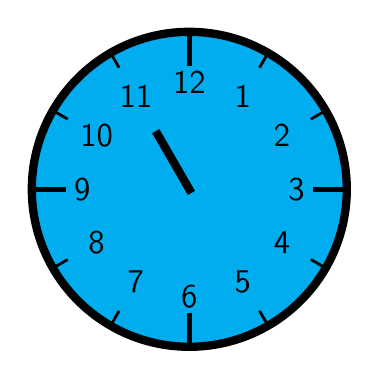
\begin{tikzpicture}[line cap=rect,line width=3pt]
\filldraw [fill=cyan] (0,0) circle [radius=2cm];
\foreach \angle [count=\xi] in {60,30,...,-270}
{
  \draw[line width=1pt] (\angle:1.8cm) -- (\angle:2cm);
  \node[font=\large] at (\angle:1.36cm) {\textsf{\xi}};
}
\foreach \angle in {0,90,180,270}
  \draw[line width=2pt] (\angle:1.6cm) -- (\angle:2cm);
\draw (0,0) -- (120:0.8cm);
\end{tikzpicture}
\]

Suppose that our clock has just an hour hand for now. Then we may collect all
the way things can be for the clock into a set of hours:
$$\Set{Hours} := \{1, 2, 3, 4, 5, 6, 7, 8, 9, 10, 11, 12\}.$$

The set $\Set{Hours}$ is the set of \emph{states} of our clock system. If we know what hour it is, we also know what hour is coming next. So, this system has the following dynamics:
%
% :CUSTOM-ID: problem-with-drawing-mapsto-nicely
%
\begin{align*}
  \fun{tick} : \Set{Hours} &\to \Set{Hours} \\
                t &\mapsto \begin{cases} t + 1 &\mbox{if $t < 12$}\\ 1 &\mbox{if $t = 12$}  \end{cases}
\end{align*}

Here's a sample of the dynamics of the clock. Say we started at 3 o'clock:
$$3 \xmapsto{\fun{tick}} 4 \xmapsto{\fun{tick}} 5 \xmapsto{\fun{tick}} 6
\xmapsto{\fun{tick}} \cdots$$

Not the most dynamic of systems, but we have to start somewhere. If we want to
refer to the whole system at once, we can box it up and write it like this:

\begin{equation}\label{eqn.clock_system_box}\tag{box1}
\begin{tikzpicture}[oriented WD, bbx = 1cm, bby =.5cm, bb min width=1cm, bb port length=4pt, bb port sep=1]
	\node[bb={1}{1}] (X) {$M$};
	\draw[label] 
		node [left=2pt of X_in1] {$A$}
		node [right=2pt of X_out1] {$B$}
		;
\end{tikzpicture}
\end{equation}

We imagine that the clock is going about its business inside the clock, and
that is shows the hour it is currently displaying on the outgoing wire.

One issue with our clock is that it doesn't tell us whether it is morning or
evening. Being morning or evening is its own way that things might be, and we
can see it as its own dynamical system. We might imagine a little addition to
our clock that reads $\const{a.m.}$ or $\const{p.m.}$:
\begin{equation}\label{eqn.whole_clock}
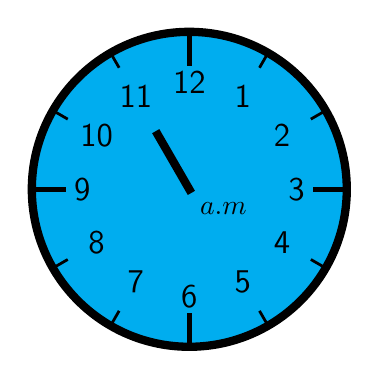
\begin{tikzpicture}[line cap=rect,line width=3pt]
\filldraw [fill=cyan] (0,0) circle [radius=2cm];
\foreach \angle [count=\xi] in {60,30,...,-270}
{
  \draw[line width=1pt] (\angle:1.8cm) -- (\angle:2cm);
  \node[font=\large] at (\angle:1.36cm) {\textsf{\xi}};
}
\foreach \angle in {0,90,180,270}
  \draw[line width=2pt] (\angle:1.6cm) -- (\angle:2cm);
\draw (0,0) -- (120:0.8cm);
\node at (330:.5cm) {$\const{a.m}$};
\end{tikzpicture}
\end{equation}

We can see this little addition as a system in its own right; it is the system
of $\const{a.m.}/\const{p.m.}$. The states of this system are
$$\Set{Meridien} = \{\const{a.m.}, \const{p.m.}\}.$$
But this time, knowing how they are going to change also requires us to know the
hour:
\begin{align*}
  \fun{next} : \Set{Meridien} \times \Set{Hours} &\to \Set{Meridien} \\
               (\const{a.m}, t) &\mapsto \begin{cases} \const{p.m.} &\mbox{if $t = 11$}\\ \const{a.m} &\mbox{otherwise}  \end{cases} \\
               (\const{p.m}, t) &\mapsto \begin{cases} \const{a.m.} &\mbox{if $t = 11$}\\ \const{p.m} &\mbox{otherwise}  \end{cases}
\end{align*}
If it is $\const{a.m.}$ and the clock reads 8, then it will still be
$\const{a.m.}$; but if it is $\const{a.m.}$ and the clock reads 11, then it will
switch on the next hour to $\const{p.m.}$.

The thing to note about the dynamics of the $\const{a.m.}/\const{p.m.}$ system
is that they depend on what hour it is. The hour is a \emph{parameter} for the
dynamics of this system. We can draw this system as a box like this:
\begin{equation}\label{eqn.am_pm_system_box}\tag{box1}
\begin{tikzpicture}[oriented WD, bbx = 1cm, bby =.5cm, bb min width=1cm, bb port length=4pt, bb port sep=1]
	\node[bb={1}{1}] (X) {$M$};
	\draw[label] 
		node [left=2pt of X_in1] {$A$}
		node [right=2pt of X_out1] {$B$}
		;
\end{tikzpicture}
\end{equation}
We have the $\Set{Meridien}$ wire coming out, which carries the information of
whether it is $\const{a.m.}$ or $\const{p.m.}$, just like the clock. But we also
have a wire coming in, which carries the hour that we need as a parameter for
our dynamics.

We can now express our whole clock (\ref{eqn.whole_clock}) by wiring together
our bare clock and the $\const{a.m.}/\const{p.m.}$ system:
\begin{equation}\label{eqn.clock_system_box}\tag{box1}
\begin{tikzpicture}[oriented WD, bbx = 1cm, bby =.5cm, bb min width=1cm, bb port length=4pt, bb port sep=1]
	\node[bb={1}{1}] (X) {$M$};
	\draw[label] 
		node [left=2pt of X_in1] {$A$}
		node [right=2pt of X_out1] {$B$}
		;
\end{tikzpicture}
\end{equation}

\end{document}
